\documentclass[../template]{subfiles}

\begin{document}
\section{Amplificatore differenziale}
\begin{center}
    \begin{tikzpicture}
        \draw
            (0, 0) node[ground]{}
            to[isource, i<=$I_D$] (0, 1.5)
            coordinate(x)
            -- ++(-1, 0)
            node[nmos, anchor=S] (nmos1){}

            (nmos1.D) to[R, l=R, i<=$I_{D1}$] ++(0, 2)
            node[vdd]{}
            (nmos1.G) node[left]{$V_{i1}$}
            (nmos1.D) -- ++(0.2, 0) node[right]{$V_{u1}$}

            (x) -- ++(1, 0)
            node[nmos, anchor=S, xscale=-1] (nmos2){}
            (nmos2.D) to[R, l=R, i<=$I_{D2}$] ++(0, 2)
            node[vdd]{}
            (nmos2.G) node[right]{$V_{i2}$}
            (nmos2.D) -- ++(0.2, 0) node[right]{$V_{u2}$}
            ;
    \end{tikzpicture}
\end{center}
\label{circuito:amplificatore_differenziale}


Da Kirchoff $I_{D1} + I_{D2} = I_D$, quindi i transistori non potranno mai essere simultaneamente spenti, altrimenti $I_D = 0$.
\begin{gather*}
    V_{i1} - V_{GS1} + V_{GS2} = V_{i2}\\
    \Downarrow\\
    V_{i1} - V_{i2} =  V_{GS1} - V_{GS2}
\end{gather*}

Di conseguenza se $V_{i1} > V_{i2}$ segue $V_{GS1} > V_{GS2}$, e siccome la corrente di drain dipende dalla tensione $V_{GS}$
allora $I_{D1} > I_{D2}$.
E siccome le tensione di uscita scritta nella forma $V_u = V_{dd} - R I_D$, ne segue che $V_{u1} < V_{u2}$.

Quindi se ai due segnali di ingresso si presenta uno sbilanciamento positivo a favore di $V_{i1}$, fra i due segnali d'uscita
si presenta uno sbilanciamento negativo rispetto a $V_{u1}$.

La somma delle correnti è limitata dal valore costante $I_D$

Se le tensioni applicate agli ingressi sono identiche, dato che il circuito è simmetrico non c'è motivo di pensare che
le correnti sui rispettivi rami non siano identiche.

Quindi:
\begin{align*}
    V_{i1} = V_{i2} \quad \Rightarrow \quad I_{D1} = I_{D2} = \frac{I_0}{2}
\end{align*}

Diversamente se le tensioni sono differenti, ci si può aspettare che scorra più corrente sul ramo a tensione maggiore.

Il caso limite si manifesta quando la differenza di tensione è talmente elevata da far circolare tutta la corrente
su un' unico ramo del circuito.


\begin{figure}[h]
    \begin{tikzpicture}
        \begin{axis}[
            ylabel={$I_{D1}, I_{D2}$},
            xlabel={$V_{i1} - V_{i2}$},
            ymin=-1,
            width=.45\textwidth
        ]

            \addplot[blue] {3 / (1 + e^(-2*x))};
            \addplot[red] {3-3 / (1 + e^(-2*x))};
            \addplot[dashed, gray]{3};
            \draw (0, 3) node[circ]{} node[left]{$I_0$};
        \end{axis}
    \end{tikzpicture}
    \begin{tikzpicture}
        \begin{axis}[
            ylabel={$V_{U1}, V_{U2}$},
            xlabel={$V_{i1} - V_{i2}$},
            ymin=-1,
            width=.45\textwidth
        ]

            \addplot[red] {.5 + 3 / (1 + e^(-2*x))};
            \addplot[blue] {.5 + 3-3 / (1 + e^(-2*x))};
            \addplot[dashed, gray]{.5};
            \draw (0, .5) node[circ]{} node[below]{$V_{dd} - R I_0$};
            \draw (0, 3.5) node[circ]{} node[above] {$V_{dd}$};
        \end{axis}
    \end{tikzpicture}

    \caption{Grafici corrente-tensione amplificatore differenziale}
    \label{fig:tensione_corrente_opamp}
\end{figure}

Intuitivamente possiamo rappresentare questo comportamento di tensione e corrente con i grafici in figura \ref{fig:tensione_corrente_opamp}.

Questo circuito guarda la differenza delle tensioni applicate agli ingressi.
A seconda della differenza frazioni della corrente circolano su un ramo o sull'altro.

Come osservabile quindi dal grafico delle tensioni di uscita, il circuito è un amplificatore che dipende dalla
differenza dei segnali d'ingresso.

Posso sempre sempre esprimere le correnti d'ingresso come la combinazione tra la componente di modo comune
$V_{ic} = \frac{V_{i1} + V_{i2}}{2}$ e la componente differenziale $V_{id} = V_{i1} - V_{i2}$.

\begin{align*}
    V_{i1} = V_{ic} + \frac{V_{id}}{2}
    \\
    V_{i2} = V_{ic} - \frac{V_{id}}{2}
\end{align*}

È possibile definire un guadagno differenziale come $A_d = \frac{dV_u}{dV_{id}}$, la variazione della tensione in uscita
in funzione della differenza di in ingresso.

Studiando il cambiamento della tensione di uscita al variare della componente di modo comune, immaginandoci di applicare
due segnali identici agli ingressi, per tenere la componente differenziale nulla, necessariamente $I_{D1} = I_{D2}$.
\\
Di conseguenza anche $V_{u1} = V_{u2}$ sono costanti se applicate le stesse variazioni di tensione ad entrambi gli ingressi.
Quindi $A_{c} = \frac{dV_u}{dV_{ic}} = 0$.

In conclusione, questo circuito amplifica la componente differenziale, ignorando completamente le variazioni di modo comune.
Per questo motivo il circuito prende il nome di "amplificatore differenziale".

\newpage
\subsection{Amplificatore operazionale ideale}
Il circuito dell'amplificatore differenziale viene espresso attraverso il seguente componente:

\begin{center}
    \begin{circuitikz}
        \draw
        (0,0) node[op amp] (opamp) {}
        (opamp.+) node[left] {$V^+$}
        (opamp.-) node[left] {$V^-$}
        (opamp.out) node[right] {$V_u$}
        ;
    \end{circuitikz}
    \qquad
    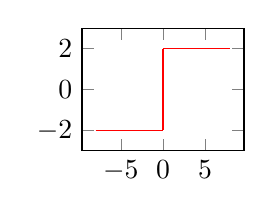
\begin{tikzpicture}
        \begin{axis}[ymax=3,ymin=-3, width=.3\textwidth]
            \addplot[red, domain=-8:0]{-2};
            \addplot[red, domain=0:8]{2};
            \addplot[red] coordinates {(0, 2) (0, -2)};
        \end{axis}
    \end{tikzpicture}
\end{center}

Rendendo il dispositivo ideale (guadagno $+\infty$), otteniamo una relazione tra tensione di ingresso e uscita
simile a quella di una funzione a gradino, esprimibile da un modello lineare a tratti:

\label{formula:ideal_opamp}
\begin{itemize}
    \item una regione di \textbf{alto guadagno}:
        \[\begin{cases}
            V_{id} = 0\\
            -V_M < V_u < V_M
        \end{cases}\]
    \item un tratto di \textbf{saturazione positiva}:
        \[\begin{cases}
            V_{u} = V_M\\
            V_{id} > 0
        \end{cases}\]
    \item ed un tratto di \textbf{saturazione negativa}:
        \[\begin{cases}
            V_{u} = -V_M\\
            V_{id} < 0
        \end{cases}\]
\end{itemize}

Per rendere compatibile questo modello ideale con il circuito dell'amplificatore differenziale risolto
precedentemente (pagina \pageref{circuito:amplificatore_differenziale}),
è necessario aumentare il guadagno, e modificare l'escursione del segnale di uscita da
$[V_{dd} - R I_0:V_M]$ a $[-V_M:+V_M]$.

Un facile trucco per poter ottenere questo risultato e mettere in serie all'uscita invertita dell'amplificatore
un invertitore polarizzato a $[-V_M:V_M]$:

\begin{center}
    \begin{circuitikz}
        \draw
        (0, 0)
        to[american current source] (0, -1.5)
            node[ground]{}
        (0, 0) -- (-1, 0)
        node[nmos, anchor=E] (n1) {}
        (n1.C) to[R] ++(0, 1.5)
        -- ++(1, 0) node[vcc](VCC){}
        (0, 0) -- (1, 0)
        node[nmos, anchor=E, xscale=-1] (n2) {}
        (n2.C) to[R] ++(0, 1.5)
            -- ++(-1, 0)
        (n1.G) node[left]{$V^+$}
        (n2.G) node[right]{$V^-$}

        (n2.C) -- ++(2, 0) coordinate(c)
        % Amplificatore mos
        % (c) - (0, 0))
        -- ++(0, -1) node[nmos, anchor=G] (ni) {}
        (ni.D) node[pmos, anchor=D] (pi) {}
        (c) -- (pi.G)

        (ni.S) node[circ]{} node[below]{$-V_M$}
        (pi.S) node[circ]{} node[above]{$V_M$}

        (ni.D) -- ++(.5, 0) node[right]{$V_u$}
        ;
    \end{circuitikz}
\end{center}

Un'ulteriore caratteristica di questo circuito è che le correnti in ingresso $I^+$ ed $I^-$ sono nulle perché
correnti di gate in ingresso a transistor nmos.

Per comportarsi in modo ideale, $V_u$ è unicamente dipendente dalla tension in ingresso $V_{id}$ ed è indipendente
da correnti e tensioni di modo comune a carico.
\\
Il circuito si deve quindi comportare come un generatore ideale di tensione , controllato dalla $V_{id}$.

Ricapitolando, le tre caratteristiche che descrivono questo componente ideale sono:
\begin{enumerate}
    \item L'uscita $V_u$ è una funzione "a gradino".
    \item Le correnti $I^+$ e $I^-$ in ingresso sono nulle.
    \item Si comporta come un generatore ideale di tensione controllato unicamente da $V_{id}$.
\end{enumerate}

\textit{Spiegazione circuito per approssimare generatore di tensione a pag. \pageref{approfondimento:approx_circuito_generatore_ideale_tensione}}

\subsection{Circuito Amplificatore invertente}

\begin{center}
    \begin{circuitikz}
        \draw (0, 0)
        node[above]{$V_i$}
        to[R, *-*, l=$R_1$, i=$I_1$] ++(2.5, 0)
        coordinate(ing1)
        -- ++(0, 1)
        to[R, l=$R_2$, i=$I_2$] ++(2.5, 0)
        coordinate(tip);
        \draw (ing1) node[op amp, anchor=-](am){};
        \draw(am.+) -- +(0, -1) node[ground]{};
        \draw(am.out) to[short, -*] ++(1, 0)
        node[right] {$V_u$};
        \draw(tip) -- (tip |- am.out);
        \draw(am.-) to[open, v>=$V_{id}$] (am.+);
    \end{circuitikz}
\end{center}

Il ramo con la resistenza $R_2$ prende il nome di ramo in retroazione, siccome collega l'uscita all'ingresso.
Ricordando le equazioni dell'amplificatore operazionale ideale (pag. \pageref{formula:ideal_opamp}), studiamo il circuito:

\subsubsection{Analisi regione di alto guadagno:}
In regione di alto guadagno, da $V_{id} = 0$ otteniamo $V^+ = V^- = 0$, in quanto la tensione $V^-$ è vincolata dal potenziale di terra, portando un riferimento di terra virtuale.
\\
Seppur il potenziale del nodo risulta a terra, non permette alla corrente di scaricarsi, dato che la corrente in ingresso è obbligatoriamente nulla.

Applicando Kirchoff: $I_1 = I_2$
\begin{align*}
    -\frac{V_u}{R_2} = \frac{V_i}{R_1}
    \quad\Rightarrow\quad
    V_u = - \frac{R_2}{R_1} V_i
\end{align*}

Rappresenta una semiretta decrescente valida per i valori di $V_i$:
\[
    -\frac{R_1}{R_2}V_M < V_i < \frac{R_1}{R_2} V_M
\]
per via dei valori di $V_u$ compresi tra $-V_M$ e $+V_M$.

Dall' equazione ottenuta possiamo osservare come è possibile variare il valore di guadagno nella regione attiva diretta,
semplicemente variando le relazioni tra le due resistenze.

\subsubsection{Analisi regione di saturazione positiva:}
Da ipotesi $V_u = V_M$, $V^+ = 0$ e $V^+ > V^-$.

L'ipotesi di cortocircuito virtuale non è più valida in quanto $V_{id} > 0$.
\\
Applicando Kirchoff $I_1 = I_2$:
\[
    \begin{rcases}
        I_1 = \frac{V_i - V^-}{R_1}\\
        I_2 = \frac{V^- - V_u}{R_2}
    \end{rcases} \Rightarrow
    V^- = \frac{V_i R_2 + V_u R_1}{R_1 + R_2}
\]

Imponendo $V^- < 0$ si ottiene la regione di validità:
\[
    V_i < - \frac{R_1}{R_2}V_M
\]

Cosa analoga accade in regione di saturazione negativa.

\begin{center}
    \begin{tikzpicture}
        \begin{axis}
            \addplot[domain=-2:2]{-x};
            \addplot[domain=2:5]{-2};
            \addplot[domain=-5:-2]{2};
        \end{axis}
    \end{tikzpicture}
\end{center}

\subsection{Amplificatore lineare non invertente}
\begin{center}
    \begin{circuitikz}
        \draw (0, 0)
        node[ground]{}
        to[R, l=$R_1$, i=$I_1$] ++(2.5, 0)
        coordinate(ing1)
        -- ++(0, 1)
        to[R, l=$R_2$, i=$I_2$] ++(2.5, 0)
        coordinate(tip);
        \draw (ing1) node[op amp, anchor=-](am){};
        \draw(am.+) to[R, l=$R_1$] ++(0, -2) node[ground]{}
            (am.+) to[R, l=$R_2$] ++(-2, 0) node[circ]{} node[below]{$V_i$};
        \draw(am.out) to[short, -*] ++(1, 0)
        node[right] {$V_u$};
        \draw(tip) -- (tip |- am.out);
        \draw(am.-) to[open, v>=$V_{id}$] (am.+);
    \end{circuitikz}
\end{center}

\subsubsection{Analisi circuito in alto guadagno:}
In regione di alto guadagno,
\begin{align*}
    &V^+ = \frac{R_2}{R_1 + R_2} V_i
    &V^- = \frac{R_1}{R_1 + R_2} V_u
\end{align*}

E da $V^+ = V^-$ si ricava il valore della tensione di uscita: $V_u = \frac{R_2}{R_1} V_i$, che è la stessa relazione di prima, ma con segno opposto.

Calcolando le condizioni di validità:
\[
    -\frac{R_1}{R_2} V_M < V_i < \frac{R_1}{R_2} V_M
    \]
\subsubsection{Regione di saturazione positiva e negativa:}
I calcoli sono gli stessi del precedente, risultando in un amplificatore lineare non invertente.

\begin{center}
    \begin{tikzpicture}
        \begin{axis}
            \addplot[domain=-2:2]{x};
            \addplot[domain=2:5]{2};
            \addplot[domain=-5:-2]{-2};
        \end{axis}
    \end{tikzpicture}
\end{center}

\subsection{Circuito sommatore analogico}
\begin{center}
    \begin{circuitikz}
        \draw (-1, 0)
        node[above]{$V_{i1}$}
        to[R, *-*, l=$R_1$] (2, 0)
        coordinate(ing1)
        -- ++(0, 1)
        to[R, l=$R_2$, i=$I_R$] ++(2.5, 0)
        coordinate(tip);
        \draw (-1, -1) node[above]{$V_{i2}$} to[R, l=$R_1$, *-] (1.5, -1) -- (1.5, 0);
        \draw (ing1) node[op amp, anchor=-](am){};
        \draw(am.+) -- +(0, -1) node[eground]{};
        \draw(am.out) to[short, -*] ++(2, 0)
        node[right] {$V_u$};
        \draw(tip) -- (tip |- am.out);
    \end{circuitikz}
\end{center}
\subsubsection{Analisi regione di alto guadagno}
In regione di alto guadagno, unendo le equazioni delle singole correnti con l'equazione di Kirchoff al nodo:
\begin{align*}
    I_1 + I_2 = \cancel{I^-} + I_R
    \\
    \frac{V_{i1} + V_{i2}}{R_1} = -\frac{V_u}{R_2}
\end{align*}
Da cui $V_u = - \frac{R_2}{R_2} (V_{i1} + V_{i2})$, risultato estremamente importante perché indica la funzione di una somma tra le due tensioni in ingresso. Per questo motivo, il circuito prende il nome di sommatore analogico.

Questo risultato ovviamente è indipendente dal numero di ingressi, e variando il valore delle resistenze legate agli ingressi è possible fare una somma pesata dei segnali in ingresso.

\subsection{Circuito derivatore}

\begin{center}
    \begin{circuitikz}
        \draw (0, 0)
        node[above]{$V_i$}
        to[C, *-*, l=$C$, i=$I_1$] ++(2.5, 0)
        coordinate(ing1)
        -- ++(0, 1)
        to[R, l=$R_2$, i=$I_2$] ++(2.5, 0)
        coordinate(tip);
        \draw (ing1) node[op amp, anchor=-](am){};
        \draw(am.+) -- +(0, -1) node[ground]{};
        \draw(am.out) to[short, -*] ++(1, 0)
        node[right] {$V_u$};
        \draw(tip) -- (tip |- am.out);
        \draw(am.-) to[open, v>=$V_{id}$] (am.+);
    \end{circuitikz}
\end{center}
\subsubsection{Analisi alto guadagno}
In regione di alto guadagno $I_R = - \frac{V_u}{R}$ e $I_C = C \frac{dV_i}{dt}$, da cui:
    \[
        V_u = -RC \frac{dV_i}{dt}
    \]

Il circuito è quindi in grado di calcolare la derivata del segnale in ingresso.

Mettendo un condensatore sul ramo di uscita ed una resistenza nel ramo in ingresso si ottiene un circuito \textbf{integratore}.

\subsection{Stadio separatore}
\begin{center}
    \begin{circuitikz}
        \draw (0, 0) node[op amp] (amp){}
        (amp.+) node[circ]{} node[left] {$V_i$}
        (amp.-) -- ++(0, 1) -| (amp.out)
        (amp.out) -- ++(0.5, 0) node[circ]{} node[above]{$V_u$}
        ;
    \end{circuitikz}
\end{center}
\begin{tcolorbox}
    In regione attiva diretta, è facile calcolare $V_u = V_i$ per $-V_M < V_i < V_M$.
\end{tcolorbox}

In questo modo è possibile leggere il valore di $V_i$ a corrente d'ingresso nulla, erogando una corrente arbitraria.
Questo principio è possibile utilizzarlo per creare un generatore di tensione
\begin{center}
    \begin{circuitikz}
    \draw (0, 0) node[ground]{}
        to[R, i<=$I_1$, l=$R_1$] (0, 2)
        to[R, i<=$I_2$, l=$R_2$] (0, 4)
        node[vdd]{}
        (0, 2) to[short, i=$I_u$] (1, 2)
        node[op amp, anchor=+] (amp){}
        (amp.-) -- ++(0, 1) -| (amp.out)

        (amp.out) to[short, i=$I_u$] ++(.5, 0){}
        node[right]{$V_u$};
    \end{circuitikz}
\end{center}
L'applicazione più importante è in strumenti di misura, essenziale per assorbire una corrente nulla dal circuito in oggetto.

\textit{Nel caso non si sia capita l'utilità di questo circuito guardare l'approfondimento a pagina \pageref{approfondimento:approx_circuito_generatore_ideale_tensione}.}

\newpage
\subsection{Trigger di Schmitt}
Ipotizzando di invertire la polarità dell'amplificatore operazionale, analizziamo il seguente circuito:

\begin{center}
    \begin{circuitikz}
        \draw (0, 0)
        node[above]{$V_i$}
        to[R, *-*, l=$R_1$, i=$I_1$] ++(2.5, 0)
        coordinate(ing1)
        -- ++(0, 1)
        to[R, l=$R_2$, i=$I_2$] ++(2.5, 0)
        coordinate(tip);
        \draw (ing1) node[op amp, anchor=+, yscale=-1](am){};
        \draw(am.-) -- +(0, -1) node[ground]{};
        \draw(am.out) to[short, -*] ++(1, 0)
        node[right] {$V_u$};
        \draw(tip) -- (tip |- am.out);
        \draw(am.+) to[open, v>=$V_{id}$] (am.-);
    \end{circuitikz}
\end{center}

\subsubsection{Analisi del circuito in regione di alto guadagno}
In regione di alto guadagno, $V^+ = V^- = 0$.
\\
Da $I_1 = I_2$:
\[
    \frac{V_i}{R_1} = - \frac{V_u}{R_2}\quad
    \Rightarrow\quad
    V_u = -\frac{R_2}{R_1} V_i
\]

Le condizioni di esistenza di rimangono le stesse:
\[
    -\frac{R_2}{R_1} V_M < V_i < \frac{R_2}{R_1} V_M
\]
\begin{tcolorbox}
La condizione $V_{id} = 0$ della regione di alto guadagno, porta ad avere risultati esattamente identici
al circuito con polarità non invertita.
\end{tcolorbox}

\subsubsection{Analisi del circuito in regione di saturazione positiva}
Da ipotesi $V_u = V_M$ e $V^+ > 0$, dato che $V^- = 0$ e $V_{id} > 0$.

Da $I_1 = I_2$:
\[
    \begin{cases}
        \frac{V_i - V^+}{R_1} = -\frac{V_M - V^+}{R_2}
        \\
        V^+ > 0
    \end{cases}
    \quad\Rightarrow\quad
    V_i > -\frac{R_1}{R_2} V_M
\]

Gli stessi calcoli possono essere svolti per la regione di saturazione negativa, ottenendo che la stessa inversione
della regione di polarità si manifesta nell'altra regione.

\subsubsection{Interpretazione dell'analisi del circuito}
Mentre la regione di alto guadagno non cambia aspetto, le regioni di saturazione invertono le regioni di funzionamento.

\begin{center}
\begin{tikzpicture}
    \begin{axis}
        \addplot[domain=-2:2]{-x};
        \addplot[domain=-5:2]{-2};
        \addplot[domain=-2:5]{2};
        \addplot[dashed, gray, thin] coordinates {(2,-5) (2, 5)};
        \addplot[dashed, gray, thin] coordinates {(-2,-5) (-2, 5)};
    \end{axis}
\end{tikzpicture}
\end{center}

La relazione tra ingresso ed uscita non è più funzionale. È richiesta una maggiore analisi per capire quale tra i tre valori
di tensione d'uscita il circuito restituisce per $-V^* < V_i < V^*$.

Ragioniamo quindi in regime dinamico, partendo da $V_a < -V^*$, spostandoci verso un punto $V_b > V^*$.
\\
Fintanto che $V_a < -V*$, il valore è univoco e costante. Raggiunto il valore critico $-V^*$, per continuità,
l'uscita si mantiene costante fino a raggiungere il punto $V^*$.
Appena raggiunto il punto $V^*$, ritorna ad essere presente un'unica soluzione, portando l'uscita al valore positivo.

\begin{center}
    \centering
    \begin{tikzpicture}
        \begin{axis}
            \addplot[thin, domain=-2:2]{-x};
            \addplot[thin, domain=-5:2]{-2};
            \addplot[thin, domain=-2:5]{2};
            \addplot[dashed, gray, thin] coordinates {(2,-5) (2, 5)};
            \addplot[dashed, gray, thin] coordinates {(-2,-5) (-2, 5)};

            \addplot[red, domain=-5:2]{-2};
            \addplot[red] coordinates {(2, -2) (2, 2)};
            \addplot[red, domain=2:5]{2};
            \draw (-4.5, 0) node[circ]{} node[above]{$V_a$};
            \draw (4.5, 0) node[circ]{} node[above]{$V_b$};
        \end{axis}
    \end{tikzpicture}
    \begin{tikzpicture}
        \begin{axis}
            \addplot[thin, domain=-2:2]{-x};
            \addplot[thin, domain=-5:2]{-2};
            \addplot[thin, domain=-2:5]{2};
            \addplot[dashed, gray, thin] coordinates {(2,-5) (2, 5)};
            \addplot[dashed, gray, thin] coordinates {(-2,-5) (-2, 5)};

            \addplot[green, domain=-5:-2]{-2};
            \addplot[green] coordinates {(-2, -2) (-2, 2)};
            \addplot[green, domain=-2:5]{2};
            \draw (-4.5, 0) node[circ]{} node[above]{$V_a$};
            \draw (4.5, 0) node[circ]{} node[above]{$V_b$};
        \end{axis}
    \end{tikzpicture}
\end{center}

Seguendo analogo ragionamento in verso opposto, si nota che per andare da $b$ ad $a$ e da $a$ a $b$, si effettuando due percorsi diversi, indicati in rosso ed in verde.
\\
Questo andamento prende il nome di ciclo di isteresi, ed il circuito prende il nome di circuito "trigger di Schmitt".

Per forzare l'uscita alta serve un valore di ingresso sufficientemente positivo.
La caratteristica di questo circuito è che si triggera, portando l'uscita ad un valore positivo.
\\
È resistente al rumore in quanto per cambiare "stato" richiede delle tensioni significative, rendendolo utile ad esempio
per un circuito dove una lampada si spegne raggiunto un certo livello di luce.

Questo è il primo circuito che presenta un elemento di memoria.

\subsection{Circuito basato su trigger di schmitt}
\begin{center}
    \begin{circuitikz}
        \draw (0, 0)
        node[ground]{}
        to[R, l=$R_1$, i=$I_1$] ++(2.5, 0)
        coordinate(ing1)
        -- ++(0, 1)
        to[R, l=$R_2$, i=$I_2$] ++(2.5, 0)
        coordinate(tip);
        \draw (ing1) node[op amp, anchor=+, yscale=-1](am){};
        \draw(am.-) -- ++(0, -.7)
        coordinate(x)
        to[C] ++(0, -1) node[ground]{}
        (x) to[R]  (x -| am.out)
        -- (am.out);
        \draw(am.out) to[short, -*] ++(1, 0)
        node[right] {$V_u$};
        \draw(tip) -- (tip |- am.out);
        \draw(am.+) to[open, v>=$V_{id}$] (am.-);
    \end{circuitikz}
\end{center}

Immaginiamo che inizialmente la capacità sia scarica, e che per un qualunque motivo, ci troviamo nella condizione di alto guadagno, con $V_u = V_M$
Ricordando che la corrente in ingresso è comunque nulla, possiamo separare il ramo e vederlo come uno risolvibile attraverso la forumla del partitore:
\begin{center}
    \begin{circuitikz}
        \draw (0, 0) node[ground]{}
        to[R] (2, 0)
        to[R] (4, 0)
        node[circ]{}
        node[right]{$V_u$}

        (2, 0) -- (2, -.5) node[below]{$V^+$};
    \end{circuitikz}
\end{center}
Quindi fintanto che $V_u = V_M$ allora
\[
    V^+ = \frac{R_q} {R_1 + R_2} V_M > 0
\]
Quindi $V_{id} > 0$, in accordo con le ipotesi. Analizzando l'altro ramo con il condensatore, siccome la tensione $V_u$ è positiva, e sul ramo circola una corrente, questa ha l'effetto di caricare il condensatore $C$, aumentando la tensione $V^-$.
Fintanto che $V_{id} > 0$, ovvero $V^+ > V^-$ allora l'amplificatore lavora in alto guadagno. Nel momento in cui $V_{id} < 0$, allora $V^- > V^+$ e l'uscita si porta con un ritardo al valore $-V_M$.

Il condensatore vedendo variato il valore di $V_u$ da $V_M$ a $-V_M$ inizia a scaricarsi, fino a quando $V^- > V_u$.
Raggiunto quel valore l'uscita si riporta a $+V_M$ e si ripete il ciclo.

Analizzando la stabilità di questo circuito infatti, il valore di $V_i = 0$, otteniamo che il circuito è instabile. In questo modo si ottiene un generatore di un segnale periodico, (onda quadra) dipendente dal valore delle resistenze e dalla capacità del condensatore.

Analogamente, mettendo a cascata un numero dispari di invertitori, e chiudendoli ad anello, si ottiene un oscillatore ad anello.

\subsection{Approssimazione circuito generatore ideale di tensione}
\label{approfondimento:approx_circuito_generatore_ideale_tensione}
Analizzando il seguente circuito:

\begin{center}
\begin{circuitikz}
    \draw (0, 0) node[ground]{}
    to[R, i<=$I_1$, l=$R_1$] (0, 2)
    to[R, i<=$I_2$, l=$R_2$] (0, 4)
    node[vdd]{}
    (0, 2) to[short, i=$I_u$] (1, 2)
    node[circ]{} node[above]{$V_u$};
\end{circuitikz}
\end{center}

Otteniamo la formula della tensione in uscita $ V_u = \frac{R_1}{R_1 + R_2} (V_{dd} - R_2 I_u) $,
da cui possiamo osservare che se la corrente in uscita $I_u$ è 0, il circuito si comporta esattamente come un partitore di corrente. Per ottenere questo risultato, colleghiamo un transistore bipolare

\begin{center}
\begin{circuitikz}
    \draw (0, 0) node[ground]{}
    to[R, i<=$I_1$, l=$R_1$] (0, 2)
    to[R, i<=$I_2$, l=$R_2$] (0, 4)
    node[vdd]{}
    (0, 2) to[short, i=$I_u$] (1, 2)
    node[npn, anchor=B] (npn){}
    (npn.C) node[vdd]{}

    (npn.E) to[short, i=$I_u$] ++(.5, 0){}
    node[right]{$V_u$};
    ;
\end{circuitikz}
\end{center}

Il quale deve necessariamente funzionare in regione attiva diretta, in quanto la corrente di emettitore $I_u > 0$ e non può essere saturo, in quanto la giunzione della base collettore è negativa.
Quindi la corrente di collettore $I_c = \beta_F I_B$ e $I_E = (\beta_F + 1) I_B$, siccome $\beta_F$ è grande, allora la corrente $I_B$ è approssimativamente 100 volte minore della corrente $I_E$. Generando una tensione in uscita pressoché indipendente dalla corrente a carico.

Le tre caratteristiche ideali di questo circuito sono che dipende unicamente dalla differenza delle tensioni in ingresso, e la tensione e corrente a carico no influiscono sull'uscita.
\end{document}

